\documentclass{article}
\usepackage[margin=3cm]{geometry}
\usepackage{graphicx}
\usepackage{listings}
\usepackage{dirtree}
\usepackage{polyglossia}
\setdefaultlanguage{italian}
\setotherlanguages{english}
\lstset{basicstyle=\ttfamily\footnotesize,breaklines=true}

\setlength\parindent{0pt}
\title{
    Analisi statica e dinamica di codice \texttt{C/C++} \\ con
    \texttt{Cppcheck} e \texttt{Valgrind} \\ \vspace{16px}
    \small Corso di Affidabilità e Sicurezza \\ dei Sistemi Software Complessi A.A. 2019/2020
}

\author{\textsc{Bernardo Giordano A18/254}}
\date{\today}

\begin{document}
\maketitle

\newpage

\tableofcontents

\newpage

%----------------------------------------------------------------------------------------
%	SECTION 1
%----------------------------------------------------------------------------------------

\section{Introduzione}

\subsection{Obiettivo}
\label{sec:obiettivo}

L'obiettivo dell'assignment è quello di approfondire le tecniche di analisi
statica e dinamica del codice \texttt{C/C++} per scoprire problemi relativi allo
scorretto utilizzo della memoria, come ad esempio mancata deallocazione (memory
leak), accesso a locazioni di memoria non valide e undefined behaviour.

In particolare, si approfondiranno i software open source \texttt{Cppcheck} e
\texttt{Valgrind} rispettivamente per l'analisi statica e quella dinamica.

\subsection{Analisi statica}
\label{sec:analisistatica}

L'analisi statica è un processo di valutazione di un sistema (in questo caso
software) o di un suo componente, volto all'analisi della sua forma, contenuto e
struttura senza che esso sia messo in esecuzione. Nella maggior parte dei casi,
l'analisi statica viene eseguita direttamente sul codice sorgente o sul codice
oggetto del programma.

L'analisi statica effettuata sul software varia a seconda del tool, in quanto
alcuni vanno a considerare solo il comportamento degli statement singoli e le
dichiarazioni di variabili all'interno di una porzione circoscritta di codice,
mentre altri vanno ad effettuare una analisi complessiva a partire dal codice
sorgente completo del programma. 

Le informazioni che si ricavano da un processo di analisi statica variano sono
molto variegate:

\begin{enumerate}
    \item highlighting di errori nel coding (sintattici o meno), come avviene
    per i tool di \emph{linting}
    \item segnalazione di variabili dichiarate e mai usate
    \item segnalazione di funzioni dichiarate e mai invocate
    \item segnalazione di memoria mai deallocata (\emph{memory leak})
    \item segnalazione di possibili loop infiniti dovuti all'irraggiungibilità
    di una o più condizioni di arresto
    \item \ldots
\end{enumerate}

L'analisi statica è una fase molto importante dello sviluppo del software (in
particolare in fase di validazione) e viene utilizzata spesso per sistemi
safety-critical e per scovare codice potenzialmente vulnerabile. Un corretto
utilizzo di questa tecnica previene l'occorrenza di errori all'interno del
software in fase di esecuzione e permette di rilasciare software in produzione
che non presenta guasti che spesso si vanno a scoprire solo con il codice in
esecuzione, quando magari è già tardi perché si sono già manifestati in fallimenti.

Tra le varie tecniche di analisi statica troviamo:

\begin{itemize}
    \item Analisi statica in compilazione: viene effettuata dal compilatore
    prima di generare il codice oggetto, per verificare caratteristiche di
    correttezza (sintattica, di coerenza tra tipi e parametri, codice non raggiungibile)
    \item Code reading: lettura individuale del codice per evidenziare
    errori/discrepanze con il progetto (tecniche basate su checklist o guidate
    dai casi d'uso)
    \item Code review: riunioni formali a cui partecipa un gruppo di persone che
    revisiona il codice allo stesso tempo
    \item Walkthrough: simulazione di casi di test eseguendo le istruzioni nel
    codice a mano
    \item Analisi del dataflow: studio del \emph{Control Flow Graph}
    \item Esecuzione simbolica: esecuzione del programma con valori simbolici
    dei dati di input invece che con valori effettivi
\end{itemize}

\subsection{Analisi dinamica}
\label{sec:analisidinamica}

L'analisi dinamica è un processo di analisi del software che prevede
l'esecuzione di un programma su un processore reale o virtuale. \\

Ci sono diverse tipologie di analisi dinamica:

\begin{itemize}
    \item Code coverage: serve a misurare il grado di utilizzo del codice
    sorgente di un programma quando viene eseguita una particolare test suite
    \item Memory error detection: serve a identificare problemi dovuti alla
    mancata deallocazione dinamica di memoria e a memory leaks.
    \item Fault localization: serve a localizzare bugs nel codice basandosi sui
    casi di test passati o falliti.
    \item Concurrency errors detection: serve a identificare condizioni di
    corsa, eccezioni e deadlock in codice multithread o concorrente.
    \item Performance analysis: il programma in esecuzione viene analizzato per
    identificare eventuali problemi prestazionali.
\end{itemize}

\subsection{Aging}
\label{sec:aging}

Con l'aging del software si fa riferimento alla tendenza dei software di
fallire, o di causare fallimenti del sistema complessivo in cui operano, quando
sono eseguiti continuamente per un certo intervallo di tempo. I fattori che
causano l'aging del software sono il memory bloating e il memory leaking, la
corruzione dei dati in memoria e il mancato rilascio di risorse richieste al
sistema operativo come gli handler dei file e delle socket. \\

Una tecnica proattiva per contrastare l'aging è la \emph{software rejuvenation},
che consiste nel rimuovere condizioni accumulate che possono portare ad errore,
anche semplicemente riavviando il software o la macchina sulla quale esso
opera. \\

Tra le cause principali dietro l'aging del software, troviamo il \emph{memory
leak}. Ogni qual volta un software in esecuzione su un sistema operativo deve
effettuare delle operazioni, esso deve richiedere blocchi di memoria per
allocare eventuali variabili e strutture dati. Quando il software termina la
propria esecuzione, il sistema operativo si aspetta che il programma abbia
liberato completamente la memoria richiesta all'avvio e durante l'esecuzione
(variabili allocate, rispettivamente, staticamente e dinamicamente). Nei
linguaggi di programmazione che prevedono un garbage collector (e.g. Java)
l'allocazione dinamica della memoria non è direttamente consentita al
programmatore e la memoria viene automaticamente liberata da un garbage
collector, che ha memoria dei riferimenti che vengono fatti ad una particolare
locazione di memoria; quando essa non viene più utilizzata dal programma, viene
liberata. In altri linguaggi come invece il C o il C++, che non hanno a
disposizione un garbage collector (in quanto, ad esempio, a differenza del Java
non operano sotto una Virtual Machine), la mancata deallocazione di memoria da
parte del programmatore può causare memory leaks. \\

È quindi importante, in fase di sviluppo, prestare la dovuta attenzione alle
allocazioni e alle deallocazioni di memoria e al suo utilizzo. Vengono incontro
a questo scopo dei tool come Cppcheck e Valgrind che sono di supporto in fase di
sviluppo per effettuare analisi statica e dinamica volta all'identificazione di
utilizzo scorretto della memoria.
 
%----------------------------------------------------------------------------------------
%	SECTION 2
%----------------------------------------------------------------------------------------

\section{Cppcheck}

\subsection{Panoramica}
\label{sec:cppcheck:panoramica}

Cppcheck è un tool per l'analisi statica di codice C e C++. Esso si concentra
sull'identificazione di undefined behaviour, utilizzo scorretto delle risorse e
costrutti potenzialmente pericolosi. Cppcheck è fatto in modo tale da avere un
numero di falsi positivi molto basso anche in condizioni di codice con sintassi
non standard e customizzata (situazione comune nei sistemi embedded).

\subsection{Installazione}
\label{sec:cppcheck:installazione}

Cppcheck può essere installato in semplicemente da un repository
che lo contiene, oppure direttamente da pacchetto. Ad esempio, su
una distribuzione Debian/Ubuntu: \\

\begin{lstlisting}[language=bash]
sudo apt install cppcheck
\end{lstlisting}

\subsection{Funzionalità}
\label{sec:cppcheck:funzionalita}

Cppcheck possiede una interfaccia grafica e una a riga di comando, a seconda
delle esigenze dell'utilizzatore. Per questo assignment, ci si concentrerà
sull'utilizzo tramite \emph{command line interface}. \\

Cppcheck è progettato affinché la data flow analysis sia \emph{bidirezionale} e non
solo \emph{forward}, come avviene per altri tool analoghi. Questo significa che
Cppcheck è in grado di diagnosticare problemi che altri tool non evidenziano.
Molti tool di analisi statica evidenzieranno questo problema di overflow della memoria:

\begin{lstlisting}[language=c]
void foo(int x) {
    int buf[10];
    if (x == 1000)
        buf[x] = 0; // <- ERRORE
}
\end{lstlisting}

Altri tool invece è in grado di diagnosticare anche problemi di overflow come il
seguente, che comportano undefined behaviour:

\begin{lstlisting}[language=c]
void foo(int x) {
    int buf[10];
    buf[x] = 0; // <- UNDEFINED BEHAVIOUR SE x >= 10
    if (x == 1000) {}
}
\end{lstlisting}

Altri esempi di undefined behaviour che Cppcheck riesce ad identificare sono i
seguenti:

\begin{itemize}
    \item Dead pointers
    \item Divisione per zero
    \item Integer overflows
    \item Operandi di bit shift invalidi
    \item Conversioni invalide
    \item Utilizzo scorretto della Standard Library
    \item Gestione della memoria
    \item Null pointer dereferences
    \item Controllo degli indici \emph{out of bounds}
    \item Uso di variabili non inizializzate
    \item Scrittura su costanti
\end{itemize}

%----------------------------------------------------------------------------------------
%	SECTION 3
%----------------------------------------------------------------------------------------

\section{Valgrind}

\subsection{Panoramica}
\label{sec:valgrind:panoramica}

Valgrind è un framework in grado di fornire una strumentazione ai binari dello spazio utente. \\

Valgrind rende disponibili un certo numero di strumenti per il profiling per il
miglioramento delle prestazioni e per una esecuzione corretta
delle applicazioni. Questi strumenti sono in grado di rilevare errori relativi
ai thread e alla memoria, permettendo
così una identificazione e correzione più semplice degli errori nel codice
dell'applicazione. Essi sono in grado di analizzare la cache, l'heap e la
previsione del branch, per identificare i fattori in grado di aumentare la
velocità dell'applicazione e ridurre l'uso della memoria. \\

Valgrind analizza l'applicazione eseguendola su una CPU sintetica, monitorandola
e misurando le prestazioni del codice esistente durante la sua esecuzione.
Successivamente stampa dei report identificando ogni processo presente
nell'esecuzione dell'applicazione su un descrittore del file specificato
dall'utente, un file, o una socket di rete. Il livello di arricchimento delle
funzioni eseguite varia in base
allo strumento di Valgrind usato e alle impostazioni, ed è importante notare
che l'esecuzione di un codice "instrumentato" può richiedere un tempo dai 4-50
volte più lungo rispetto al tempo di esecuzione normale. \\

Valgrind può essere usato sulle applicazioni senza alcuna ricompilazione
aggiuntiva. Tuttavia, poichè Valgrind utilizza informazioni di debugging per
definire le problematiche nel codice, se l'applicazione e le librerie di
supporto non sono state compilate con informazioni di debugging abilitate, è
generalmente consigliato ricompilare l'applicazione in modalità di debug.

\subsection{Installazione}
\label{sec:valgrind:installazione}

Il framework Valgrind può essere installato in semplicemente da un repository
che lo contiene, oppure direttamente da pacchetto. Ad esempio, su
una distribuzione Debian/Ubuntu: \\

\begin{lstlisting}[language=bash]
sudo apt install valgrind
\end{lstlisting}

Generalmente, Valgrind viene eseguito nel seguente modo:

\begin{lstlisting}[language=bash]
valgrind --tool=toolname program
\end{lstlisting}
dove \texttt{toolname} è il nome dello strumento di Valgrind desiderato, e
\texttt{program} è il nome del programma desiderato da usare con Valgrind.

\subsection{Funzionalità}
\label{sec:valgrind:funzionalita}

La suite Valgrind contiene al suo interno un vasto assortimento di strumenti di
debugging e profiling.

\subsubsection{Memcheck}

Memcheck rileva i problemi di gestione della memoria ed è
rivolto principalmente ai programmi C e C++. Quando un programma viene eseguito
sotto la supervisione di Memcheck, tutte le letture e le scritture della memoria
vengono controllate e le chiamate a \texttt{malloc}, \texttt{new}, \texttt{free}
e \texttt{delete} vengono intercettate. Di conseguenza, Memcheck può rilevare se
il programma:

\begin{itemize}
    \item Accede a memoria che non dovrebbe (aree non ancora allocate, aree che
    sono state liberate, aree oltre la fine dei blocchi di heap, aree inaccessibili dello stack).
    \item Utilizza valori non inizializzati.
    \item Perde memoria.
    \item Esegue liberazioni errate di blocchi di heap (double free).
    \item Passa blocchi di memoria di origine e destinazione sovrapposti a \texttt{memcpy}
    e alle funzioni correlate.
\end{itemize}

Memcheck segnala questi errori non appena si verificano, fornendo il numero di
riga di origine in cui si è verificato e anche una traccia dello stack delle
funzioni chiamate per raggiungere quella riga. Memcheck tiene traccia
dell'indirizzabilità a livello di byte e dell'inizializzazione dei valori a
livello di bit. Di conseguenza, è in grado di rilevare l'uso di singoli bit non
inizializzati.
Memcheck esegue programmi circa 10-30 volte più lentamente del normale. \\

Gli errori precedentemente menzionati vengono solo segnalati da Memcheck, che
non impedisce la loro generazione. Se un programma esegue un accesso alla
memoria che genera un errore di segmentazione, questo errore si verificherà anche se
si utilizza Memcheck. Detto questo, Memcheck registrerà un messaggio
immediatamente prima dell'errore. \\

Memcheck fornisce diverse opzioni a riga di comando per rendere l'analisi più flessibile. Alcune di queste opzioni sono:

\begin{description}
    \item[\texttt{--leak-check}] Se abilitato Memcheck va alla ricerca di perdite di memoria
    quando il programma termina la sua esecuzione. Il valore predefinito è
    \texttt{summary}, e il suo output riporta il numero di perdite trovate. Altri valori
    possibili sono \texttt{yes} e \texttt{full}, entrambi riportano le informazioni su ogni perdita
    individuale e \texttt{no} disabilita questo tipo di controllo.

    \item[\texttt{--undef-value-errors}] Se abilitato (impostato su \texttt{yes}), Memcheck riporta gli errori se vengono
    usati valori non identificati. Se disabilitato (impostato su \texttt{no}), questi
    errori non vengono riportati. Questa opzione è abilitata per impostazione
    predefinita. La sua disabilitazione aumenta leggermente la velocità di
    esecuzione di Memcheck.
\end{description}

\subsubsection{Cachegrind}

Cachegrind è un profiler della cache. Esegue una simulazione dettagliata delle
cache L2 nella CPU e quindi può individuare con precisione le fonti di
\emph{cache miss} nel codice. Identifica il numero di cache miss, riferimenti di
memoria e istruzioni eseguite per ogni riga di codice sorgente, con riepiloghi
per funzione, per modulo e per l'intero programma. È utilizzabile con programmi scritti
in qualsiasi linguaggio. Cachegrind esegue i programmi circa 20-100 volte più
lentamente del normale. \\

Cachegrind è in grado di ottenere le seguenti informazioni per l'intero programma e per ogni funzione presente al suo interno:

\begin{itemize}
    \item Richieste di lettura non eseguite (read misses) e lettura (o
    istruzioni eseguite) delle istruzioni per cache del primo livello, e
    richieste di lettura non eseguite per le istruzioni della cache dell'ultimo livello.
    \item Lettura dati della cache (o lettura della memoria), richieste di lettura non eseguite.
    \item Scrittura dati della cache (o scrittura della memoria), richieste di scrittura non eseguite.
    \item Branch condizionali eseguiti e previsti incorrettamente.
    \item Branch indiretti eseguiti e previsti incorrettamente.
\end{itemize}

Per impostazione predefinita Cachegrind stampa un sommario delle informazioni
relative alle statistiche sopra riportate, e scrive in modo più dettagliato le
informazioni sul profiling su un file (\texttt{cachegrind.out.pid}, dove \texttt{pid} è l'ID del
processo del programma sul quale è stato eseguito Cachegrind). \\

Alcune opzioni da riga di comando per rendere l'analisi più flessibile sono le
seguenti:

\begin{description}
    \item[\texttt{--cache-sim}] Abilita o disabilita la raccolta dei conteggi relativi al mancato accesso e dell'accesso della cache. Il valore predefinito è \texttt{yes} (abilitato).
    \item[\texttt{--branch-sim}] Abilita o disabilita la raccolta delle informazioni relative ai conteggi
    previsti incorrettamente e sulle istruzioni del branch. Per impostazione
    predefinita questa opzione è impostata su \texttt{no} (disabilitato), poichè
    rallenterà Cachegrind di circa il 25 per cento. 
\end{description}

Callgrind è un tool aggiuntivo che nasce come estensione di Cachegrind, che
fornisce informazioni aggiuntive sui call graphs.

\subsubsection{Massif}

Massif è un profiler della memoria heap. Esegue una profilazione dettagliata dell'heap
acquisendo istantanee regolari dell'heap di un programma. Produce un grafico che
mostra l'utilizzo dell'heap nel tempo, comprese le informazioni su quali parti
del programma sono responsabili della maggior parte delle allocazioni di
memoria. Il grafico è integrato da un file di testo o HTML che include ulteriori
informazioni per determinare dove viene allocata la maggior parte della memoria.
Massif esegue programmi circa 20 volte più lentamente del normale. \\

I dati sul profiling raccolti da Massif vengono scritti su un file che per
impostazione predefinita viene chiamato \texttt{massif.out.pid}, dove \texttt{pid} è l'ID del processo del programma specificato.
Questi dati possono essere rappresentati in modo grafico con il comando \texttt{ms\_print}.

\begin{lstlisting}[language=bash]
ms_print massif.out.pid
\end{lstlisting}

Così facendo verrà generato un grafico sul consumo della memoria relativa
all'esecuzione del programma. \\

Massif fornisce un certo numero di opzioni della linea di comando utilizzabili.
Alcune opzioni disponibili sono: 

\begin{description}
    \item[\texttt{--heap}] Specifica se eseguire il profiling di heap. Il valore predefinito è \texttt{yes}. Il profiling di heap può essere disabilitato impostando questa opzione su \texttt{no}. 
    \item[\texttt{--heap-admin}] Specifica il numero di byte per blocco da usare per la gestione quando il profiling di heap è abilitato. Il valore predefinito è 8 byte per blocco.
    \item[\texttt{--stacks}] Specifica se eseguire il profiling dello stack. Il
    valore predefinito è \texttt{no} (disabilitato). Per abilitare il profiling
    dello stack bisogna impostare questa opzione su yes, ma in questo modo verrà sensibilmente rallentata l'esecuzione di Massif. Da
    notare che Massif assume che la dimensione dello stack sia zero
    all'avvio.
    \item[\texttt{--time-unit}] Specifica l'unità di tempo usata per il profiling. Sono disponibili tre
    valori validi per questa opzione: istruzioni eseguite (\texttt{i}), il valore
    predefinito, che risulta utile in numerosi casi; real time (\texttt{ms}, in
    millisecondi), utile in determinate situazioni; e byte allocati/deallocati
    sull'heap/o stack (\texttt{B}), utile per programmi eseguiti brevemente e per
    l'esecuzione di test, poichè questo processo risulta essere quello più
    facilmente riproducibile su diverse macchine. Questa opzione è utile per un
    grafico dell'output di Massif con \texttt{ms\_print}. 
\end{description}


\subsubsection{Helgrind}

Helgrind è un debugger di thread che trova race conditions in programmi
multithread. Cerca le posizioni di memoria a cui si accede da più di un thread
(POSIX o pthread), ma per le quali non è possibile trovare alcun blocco
utilizzato in modo coerente. Tali posizioni sono indicative
della mancata sincronizzazione tra i thread e potrebbero causare problemi
dipendenti dalla temporizzazione altrimenti difficili da trovare. È utile per qualsiasi
programma che utilizza i pthreads.

\subsubsection{DRD}

DRD è uno strumento per rilevare errori nei programmi C e C++ multithread. Lo
strumento funziona per qualsiasi programma che utilizza le primitive di
threading POSIX o che utilizza concetti di threading costruiti sopra le
primitive di threading POSIX. Sebbene Helgrind possa rilevare le violazioni
dell'ordine di blocco, per la maggior parte dei programmi DRD necessita di meno
memoria per eseguire la sua analisi, e quindi può essere considerato come
un'alternativa.

\subsubsection{DHAT}

DHAT è uno strumento per esaminare come i programmi utilizzano le allocazioni di
heap. Tiene traccia dei blocchi allocati e ispeziona ogni accesso alla memoria
per trovare quale blocco deve essere allocato. Viene fornito con una GUI per
facilitare l'esplorazione dei risultati di profiling.

%----------------------------------------------------------------------------------------
%	SECTION 4
%----------------------------------------------------------------------------------------

\newpage
\section{Esempi di utilizzo}

\subsection{Caso 1: memory leak, out of bounds read, read after free, double free}
\label{sec:caso1}

\begin{lstlisting}[language=c]
#include <stdlib.h>
#include <stdio.h>

int main() {
    int* buffer1 = malloc(100 * sizeof(int));
    int* buffer2 = malloc(100 * sizeof(int));
    int* buffer3 = malloc(100 * sizeof(int));

    int a = buffer1[0];
    int b = buffer1[102];

    free(buffer1);
    free(buffer3);

    int c = buffer1[0];
    printf("%d\n", c);

    free(buffer3);
    return 0;
}
\end{lstlisting}

Questo codice effettua tre allocazioni dinamiche di 400 byte ciascuna, dopodiché
effettua una \emph{out of bounds read} per definire la variabile \texttt{b}.
Successivamente \texttt{buffer1} viene deallocato con una \texttt{free} e viene
nuovamente letto per definire la variabile \texttt{c}. Infine, \texttt{buffer2}
non viene mai deallocato. \texttt{buffer3} viene invece deallocato
scorrettamente due volte. \\

Eseguendo Cppcheck:

\begin{lstlisting}[language=bash]
$ cppcheck main.c 
Checking main.c ...
main.c:10:20: error: Array 'buffer1[100]' accessed at index 102, which is out of bounds. [arrayIndexOutOfBounds]
    int b = buffer1[102];
                   ^
main.c:15:13: error: Dereferencing 'buffer1' after it is deallocated / released [deallocuse]
    int c = buffer1[0];
            ^
main.c:18:5: error: Memory pointed to by 'buffer3' is freed twice. [doubleFree]
    free(buffer3);
    ^
main.c:13:5: note: Memory pointed to by 'buffer3' is freed twice.
    free(buffer3);
    ^
main.c:18:5: note: Memory pointed to by 'buffer3' is freed twice.
    free(buffer3);
    ^
main.c:19:5: error: Memory leak: buffer2 [memleak]
    return 0;
    ^
\end{lstlisting}

Eseguendo Valgrind:

\begin{lstlisting}[language=bash]
$ valgrind -s --leak-check=full ./a.out 
==11225== Memcheck, a memory error detector
...
==11225== HEAP SUMMARY:
==11225==     in use at exit: 400 bytes in 1 blocks
==11225==   total heap usage: 4 allocs, 4 frees, 2,224 bytes allocated
==11225== 
==11225== 400 bytes in 1 blocks are definitely lost in loss record 1 of 1
==11225==    at 0x483B7F3: malloc 
==11225==    by 0x1091AC: main 
==11225== 
==11225== LEAK SUMMARY:
==11225==    definitely lost: 400 bytes in 1 blocks
==11225==    indirectly lost: 0 bytes in 0 blocks
==11225==      possibly lost: 0 bytes in 0 blocks
==11225==    still reachable: 0 bytes in 0 blocks
==11225==         suppressed: 0 bytes in 0 blocks
==11225== 
==11225== ERROR SUMMARY: 4 errors from 4 contexts (suppressed: 0 from 0)
==11225== 
==11225== 1 errors in context 1 of 4:
==11225== Invalid free() / delete / delete[] / realloc()
==11225==    at 0x483CA3F: free 
==11225==    by 0x109217: main 
==11225==  Address 0x4a5e3e0 is 0 bytes inside a block of size 400 free'd
==11225==    at 0x483CA3F: free 
==11225==    by 0x1091EC: main 
==11225==  Block was alloc'd at
==11225==    at 0x483B7F3: malloc 
==11225==    by 0x1091BA: main 
==11225== 
==11225== 
==11225== 1 errors in context 2 of 4:
==11225== Invalid read of size 4
==11225==    at 0x1091F1: main 
==11225==  Address 0x4a5e040 is 0 bytes inside a block of size 400 free'd
==11225==    at 0x483CA3F: free 
==11225==    by 0x1091E0: main 
==11225==  Block was alloc'd at
==11225==    at 0x483B7F3: malloc 
==11225==    by 0x10919E: main 
==11225== 
==11225== 
==11225== 1 errors in context 3 of 4:
==11225== Invalid read of size 4
==11225==    at 0x1091CC: main 
==11225==  Address 0x4a5e1d8 is 8 bytes after a block of size 400 alloc'd
==11225==    at 0x483B7F3: malloc 
==11225==    by 0x10919E: main 
==11225== 
==11225== ERROR SUMMARY: 4 errors from 4 contexts (suppressed: 0 from 0)
\end{lstlisting}

Cppcheck riconosce gli errori previsti compreso il double free. Valgrind non riconosce la lettura
successiva alla deallocazione della memoria. In compenso, fornisce una analisi
dettagliata dell'utilizzo della memoria, restituendo gli indirizzi invalidi e
l'ammontare di heap che non è stato liberato (400 bytes come previsto).

\newpage
\subsection{Caso 2: memory leak, allocation/deallocation mismatching}
\label{sec:caso2}

\begin{lstlisting}[language=c++]
#include <stdlib.h>

class Foo {
private:
    char* str1;
    char* str2;
    char* str3;
public:
    Foo();
    ~Foo();
};
Foo::Foo() {
    str1 = new char[10];
    str2 = new char[10];
    str3 = new char[10];
}
Foo::~Foo() {
    free(str1);
    delete[] str2;
}

int main() {
    Foo* bar = new Foo();
    delete bar;
    return 0;
}
\end{lstlisting}

Questo programma C++ mostra una classe con tre attributi di tipo puntatore a
carattere, che vengono allocati dinamicamente nel costruttore con una
\texttt{new}. \\
Il distruttore dealloca correttamente \texttt{str2}, non dealloca affatto
\texttt{str1} ed effettua la deallocazione di \texttt{str1} con la funzione
sbagliata (\texttt{free} invece di \texttt{delete}). \\

Eseguendo Cppcheck, viene evidenziato solo l'errore di programmazione relativo
all'errore in fase di deallocazione di \texttt{str1}. Non viene quindi
evidenziato il memory leak su \texttt{str3}.

\begin{lstlisting}[language=bash]
$ cppcheck main.cpp 
Checking main.cpp ...
main.cpp:20:5: error: Mismatching allocation and deallocation: Foo::str1 [mismatchAllocDealloc]
    free(str1);
    ^
\end{lstlisting}

Eseguendo Valgrind:

\begin{lstlisting}[language=bash]
$ valgrind -s --leak-check=full ./a.out 
==8222== Memcheck, a memory error detector
...
==8222== HEAP SUMMARY:
==8222==     in use at exit: 10 bytes in 1 blocks
==8222==   total heap usage: 5 allocs, 4 frees, 72,758 bytes allocated
==8222== 
==8222== 10 bytes in 1 blocks are definitely lost in loss record 1 of 1
==8222==    at 0x483C583: operator new[](unsigned long) 
==8222==    by 0x10922C: Foo::Foo() 
==8222==    by 0x10929E: main 
==8222== 
==8222== LEAK SUMMARY:
==8222==    definitely lost: 10 bytes in 1 blocks
==8222==    indirectly lost: 0 bytes in 0 blocks
==8222==      possibly lost: 0 bytes in 0 blocks
==8222==    still reachable: 0 bytes in 0 blocks
==8222==         suppressed: 0 bytes in 0 blocks
==8222== 
==8222== ERROR SUMMARY: 2 errors from 2 contexts (suppressed: 0 from 0)
==8222== 
==8222== 1 errors in context 1 of 2:
==8222== Mismatched free() / delete / delete []
==8222==    at 0x483CA3F: free 
==8222==    by 0x10925A: Foo::~Foo() 
==8222==    by 0x1092B3: main 
==8222==  Address 0x4dbcce0 is 0 bytes inside a block of size 10 alloc'd
==8222==    at 0x483C583: operator new[](unsigned long) 
==8222==    by 0x109203: Foo::Foo() 
==8222==    by 0x10929E: main 
==8222== 
==8222== ERROR SUMMARY: 2 errors from 2 contexts (suppressed: 0 from 0)
\end{lstlisting}

Valgrind evidenzia correttamente entrambi gli errori presenti nel codice,
mostrando quindi anche il fatto che 10 bytes si siano persi perché mai
deallocati. \\
Interessante notare come per questo programma molto semplice, nel quale vengono
allocati esplicitamente solo 30 bytes, ne vengono in realtà allocati
complessivamente 72758 dalle routine interne di C++, per poi venire deallocati. 

\newpage
\subsection{Caso 3: memory leak causato dal cattivo uso di \texttt{realloc}}
\label{sec:caso3}

\begin{lstlisting}[language=c]
#include <stdio.h>
#include <stdlib.h>

void foo() {
    static char* buf = 0;
    if ((buf = realloc(buf, 100)) == NULL)
        return;
    free(buf);
}

int main() {
    foo();
    return 0;
}
\end{lstlisting}

Questo programma presenta un memory leak in quanto in caso di fallimento
di \texttt{realloc}, il puntatore di \texttt{buf} verrà settato a \texttt{NULL}
ma la memoria non sarà rilasciata.

Eseguendo cppcheck:

\begin{lstlisting}[language=bash]
$ cppcheck main.c
Checking main.c ...
main.c:6:10: error: Common realloc mistake: 'buf' nulled but not freed upon failure [memleakOnRealloc]
    if ((buf = realloc(buf, 100)) == NULL)
         ^
\end{lstlisting}

Eseguendo Valgrind, invece, l'errore viene riconosciuto solo quando
\texttt{realloc} effettivamente fallisce. In questa esecuzione infatti, esso non
viene riconosciuto.

\begin{lstlisting}[language=bash]
$ valgrind -s --leak-check=full ./a.out 
==7348== Memcheck, a memory error detector
...
==7348== HEAP SUMMARY:
==7348==     in use at exit: 0 bytes in 0 blocks
==7348==   total heap usage: 1 allocs, 1 frees, 100 bytes allocated
==7348== 
==7348== All heap blocks were freed -- no leaks are possible
==7348== 
==7348== ERROR SUMMARY: 0 errors from 0 contexts (suppressed: 0 from 0)
\end{lstlisting}

Con questo esempio si evidenzia l'importanza dell'esecuzione dell'analisi
statica, perché problemi simili non sempre vengono riconosciuto immediatamente
tramite l'analisi dinamica.

\newpage
\subsection{Caso 4: undefined behaviour}
\label{sec:caso4}

\begin{lstlisting}[language=c]
#include <stdio.h>

int main(int argc, char** argv) {
    char buffer[10];
    if (argc == 2) {
        sprintf(buffer, "%s", argv[1]);
    }
    printf("%s\n", buffer);
    return 0;
}
\end{lstlisting}

Il seguente codice può presentare undefined behaviour se al programma non
vengono passati parametri (o ne viene passato più di uno), in quanto viene
stampato un buffer di caratteri non inizializzato in output. Inoltre, il
programma presenta codice non sicuro in quanto viene utilizzata la funzione
\texttt{sprintf} invece che la sua variante più safe \texttt{snprintf}, che
permette di specificare quanti byte scrivere nel buffer destinazione. In questo
caso, se come parametro al programma viene passato un argomento più lungo di 10
caratteri, si verificherà uno stack smashing in esecuzione. \\

Compilo il codice con \texttt{gcc main.c}. \\

Lo eseguo passando come parametro una stringa più lunga di 10 caratteri:

\begin{lstlisting}[language=bash]
$ ./a.out testtesttest
testtesttest
*** stack smashing detected ***: terminated
Annullato (core dump creato)
\end{lstlisting}

Cppcheck non è in grado di rilevare l'errore, se viene invocato \texttt{cppcheck
main.c}. \\

Valgrind restituisce un output più dettagliato e rileva gli errori previsti da
questo caso di studio.

\begin{lstlisting}[language=bash]
$ valgrind --track-origins=yes -s ./a.out 
==14564== Memcheck, a memory error detector
...
==14564== ERROR SUMMARY: 1 errors from 1 contexts 
==14564== 
==14564== 1 errors in context 1 of 1:
==14564== Conditional jump or move depends on uninitialised value(s)
==14564==    at 0x483EF49: strlen
==14564==    by 0x48F05B3: puts
==14564==    by 0x1091DF: main
==14564==  Uninitialised value was created by a stack allocation
==14564==    at 0x109189: main
==14564== 
==14564== ERROR SUMMARY: 1 errors from 1 contexts 
\end{lstlisting}

\begin{lstlisting}[language=bash]
$ valgrind --track-origins=yes -s ./a.out testtesttest
==14672== Memcheck, a memory error detector
...
==14672== Command: ./a.out testtesttest
==14672== 
testtesttest
*** stack smashing detected ***: terminated
==14672== 
==14672== Process terminating with default action of signal 6 (SIGABRT)
==14672==    at 0x48AF18B: raise (raise.c:51)
==14672==    by 0x488E858: abort (abort.c:79)
==14672==    by 0x48F93ED: __libc_message (libc_fatal.c:155)
==14672==    by 0x499BB49: __fortify_fail (fortify_fail.c:26)
==14672==    by 0x499BB15: __stack_chk_fail (stack_chk_fail.c:24)
==14672==    by 0x1091F8: main
==14672== 
==14672== HEAP SUMMARY:
==14672==     in use at exit: 0 bytes in 0 blocks
==14672==   total heap usage: 1 allocs, 1 frees, 1,024 bytes allocated
==14672== 
==14672== All heap blocks were freed -- no leaks are possible
==14672== 
==14672== ERROR SUMMARY: 0 errors from 0 contexts 
Annullato (core dump creato)
\end{lstlisting}

In caso di stack smashing, l'esecuzione del programma viene interrotta ma
Valgrind gestine in maniera robusta il fallimento e termina correttamente
mostrando lo stacktrace che ha portato alla generazione del fallimento.

\newpage
\subsection{Caso 5: memory leak dovuto all'utilizzo scorretto di funzioni di libreria}
\label{sec:caso5}

\begin{lstlisting}[language=c]
#include <string.h>

int main() {
    const char* src = "ASSSC";
    char* dst = strdup(src);
    return 0;
}
\end{lstlisting}

Questo semplice programma duplica una stringa di caratteri utilizzando la
funzione di libreria \texttt{strdup}. Questa funzione alloca internamente (e dinamicamente) la
memoria necessaria a contenere la copia della stringa sorgente (quindi in questo
caso 5 caratteri più un carattere terminatore), ma non la dealloca, perché è un
compito che spetta al programmatore. In questo programma la memoria non viene
deallocata esplicitamente con una \texttt{free}.

Eseguendo Cppcheck, l'errore non viene evidenziato. \\

Eseguendo Valgrind, l'errore viene evidenziato e il programma indica che sono
stati persi complessivamente 6 bytes.

\begin{lstlisting}[language=bash]
$ valgrind -s --leak-check=full ./a.out 
==8940== Memcheck, a memory error detector
...
==8940== HEAP SUMMARY:
==8940==     in use at exit: 6 bytes in 1 blocks
==8940==   total heap usage: 1 allocs, 0 frees, 6 bytes allocated
==8940== 
==8940== 6 bytes in 1 blocks are definitely lost in loss record 1 of 1
==8940==    at 0x483B7F3: malloc 
==8940==    by 0x490B50E: strdup (strdup.c:42)
==8940==    by 0x10916B: main 
==8940== 
==8940== LEAK SUMMARY:
==8940==    definitely lost: 6 bytes in 1 blocks
==8940==    indirectly lost: 0 bytes in 0 blocks
==8940==      possibly lost: 0 bytes in 0 blocks
==8940==    still reachable: 0 bytes in 0 blocks
==8940==         suppressed: 0 bytes in 0 blocks
==8940== 
==8940== ERROR SUMMARY: 1 errors from 1 contexts (suppressed: 0 from 0)
\end{lstlisting}

\newpage
\subsection{Caso 6: null pointer dereference}
\label{sec:caso6}

\begin{lstlisting}[language=c++]
int main() {
    char* c = (char*)"ASSSC";
    char* d = 0;
    /* ... codice ... */
    delete c;
    delete d;
    c[0] = 0;
    d[0] = 0;
    return 0;
}
\end{lstlisting}

In questo programma C++ vengono definite due stringhe di caratteri, una che
punta ad un valore costante e una a \texttt{nullptr}. Si suppone che ci sia del
codice utile prima delle \texttt{delete}. \texttt{delete c;} è una operazione
scorretta in quanto il valore di \texttt{c} viene assegnato nello stack nella
prima riga del main. Si suppone che per \texttt{d} il valore venga assegnato
dinamicamente nel codice omesso per brevità. Il programma successivamente tenta
di effettuare due scritture su \texttt{c} e \texttt{d}, causando una null
pointer dereference. 

Eseguendo Cppcheck, viene evidenziata la null pointer dereference su \texttt{d}.
Viene inoltre segnalato un undefined behaviour, in quanto non è una \emph{best
practice} modificare direttamente o indirettamente il valore di una stringa
nella maniera adottata dal programma.

\begin{lstlisting}[language=bash]
$ cppcheck main.cpp 
Checking main.cpp ...
main.cpp:8:5: error: Null pointer dereference: d [nullPointer]
    d[0] = 0;
    ^
main.cpp:3:15: note: Assignment 'd=0', assigned value is 0
    char* d = 0;
              ^
main.cpp:2:22: error: Modifying string literal "ASSSC" directly or indirectly is undefined behaviour. [stringLiteralWrite]
    char* c = (char*)"ASSSC";
                     ^
main.cpp:7:5: note: Modifying string literal "ASSSC" directly or indirectly is undefined behaviour.
    c[0] = 0;
    ^
\end{lstlisting}

Eseguendo Valgrind, viene segnalata l'operazione di \texttt{delete} scorretta
effettuata sulla variabile \texttt{c}, che non si trova nell'heap.

\begin{lstlisting}[language=bash]
$ valgrind -s --leak-check=full ./a.out 
==9894== Memcheck, a memory error detector
...
==9894== HEAP SUMMARY:
==9894==     in use at exit: 0 bytes in 0 blocks
==9894==   total heap usage: 1 allocs, 2 frees, 72,704 bytes allocated
==9894== 
==9894== All heap blocks were freed -- no leaks are possible
==9894== 
==9894== ERROR SUMMARY: 1 errors from 1 contexts (suppressed: 0 from 0)
==9894== 
==9894== 1 errors in context 1 of 1:
==9894== Invalid free() / delete / delete[] / realloc()
==9894==    at 0x483D1CF: operator delete(void*, unsigned long) 
==9894==    by 0x10917D: main 
==9894==  Address 0x10a004 is in a r-- mapped file a.out segment
==9894== 
==9894== ERROR SUMMARY: 1 errors from 1 contexts (suppressed: 0 from 0)
\end{lstlisting}

\newpage
\subsection{Caso 7: resource leak}
\label{sec:caso7}

\begin{lstlisting}[language=c]
#include <stdio.h>

int main() {
    FILE* file = fopen("main.c", "r");
    if (!file) {
        /* error handling */
        return 0;
    }
    return 0;
}
\end{lstlisting}

Questo programma apre un file e non rilascia l'handler alla risorsa al termine dell'esecuzione, causando un
resource leak. \\

Cppcheck riconosce correttamente l'errore.

\begin{lstlisting}[language=bash]
$ cppcheck main.c 
Checking main.c ...
main.c:9:5: error: Resource leak: file [resourceLeak]
    return 0;
    ^
\end{lstlisting}

Valgrind riconosce l'errore così come Cppcheck, ma questo non viene
immediatamente evidenziato se non specificando \texttt{--show-leak-kinds=all}
come parametro.

\begin{lstlisting}[language=bash]
$ valgrind -s --leak-check=full --show-leak-kinds=all ./a.out 
==12959== Memcheck, a memory error detector
...
==12959== HEAP SUMMARY:
==12959==     in use at exit: 472 bytes in 1 blocks
==12959==   total heap usage: 1 allocs, 0 frees, 472 bytes allocated
==12959== 
==12959== 472 bytes in 1 blocks are still reachable in loss record 1 of 1
==12959==    at 0x483B7F3: malloc 
==12959==    by 0x48EEAAD: __fopen_internal (iofopen.c:65)
==12959==    by 0x48EEAAD: fopen@@GLIBC_2.2.5 (iofopen.c:86)
==12959==    by 0x109167: main 
==12959== 
==12959== LEAK SUMMARY:
==12959==    definitely lost: 0 bytes in 0 blocks
==12959==    indirectly lost: 0 bytes in 0 blocks
==12959==      possibly lost: 0 bytes in 0 blocks
==12959==    still reachable: 472 bytes in 1 blocks
==12959==         suppressed: 0 bytes in 0 blocks
==12959== 
==12959== ERROR SUMMARY: 0 errors from 0 contexts (suppressed: 0 from 0)
\end{lstlisting}

%----------------------------------------------------------------------------------------
%	SECTION 5
%----------------------------------------------------------------------------------------

\newpage
\section{Casi studio complessi}

\subsection{Caso di studio: Checkpoint}
\label{sec:checkpoint}

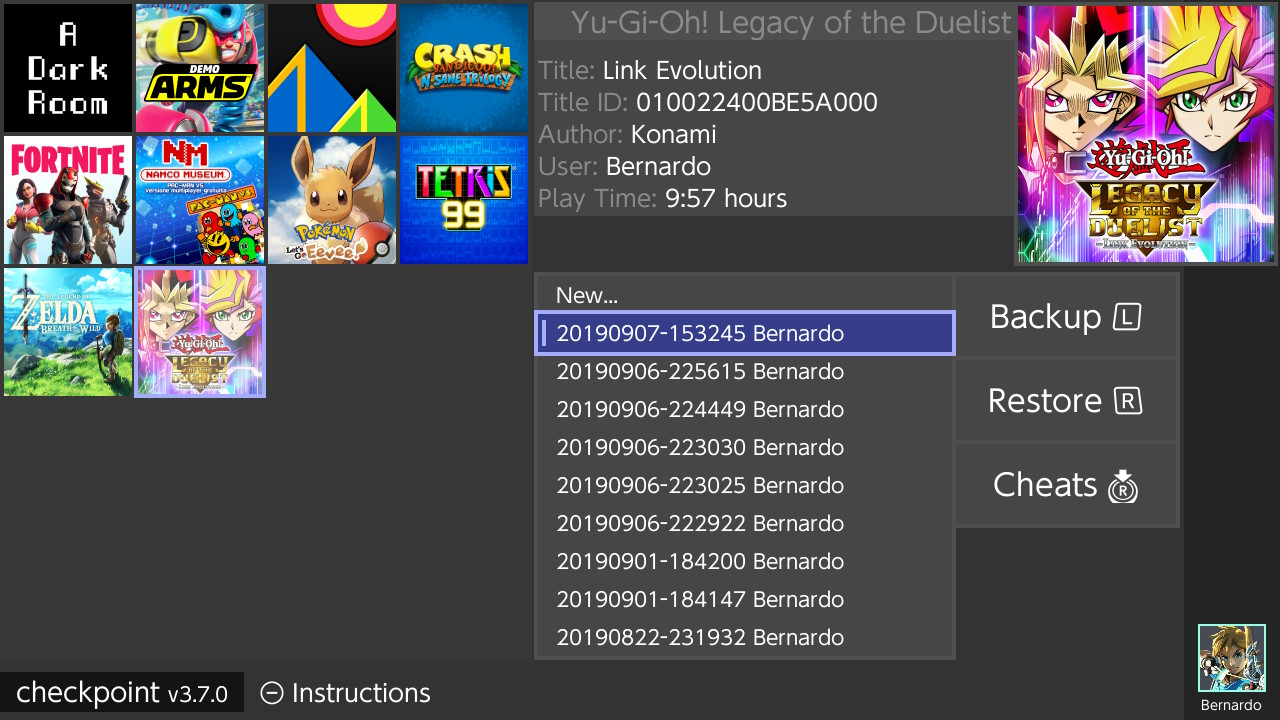
\includegraphics[width=0.68\textwidth]{images/checkpoint1.jpeg}
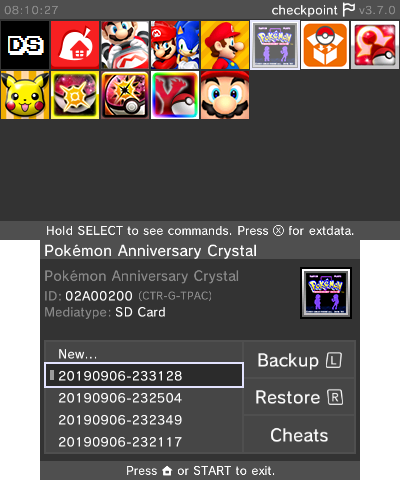
\includegraphics[width=0.32\textwidth]{images/checkpoint2.png}

Come esempio di software più realistico, scelgo di utilizzare il codice sorgente
di un mio vecchio software scritto per essere eseguito su piattaforma Nintendo
3DS e Nintendo Switch, \texttt{Checkpoint}. Checkpoint è un gestore di
salvataggi che permette estrazione e ripristino da e verso la memoria interna
della console. Il software è scritto in \texttt{C++} e per praticità si
proseguirà solo all'analisi statica, in quanto non è possibile eseguire Valgrind
direttamente sull'hardware destinazione. \\

Entrambi i programmi prevedono l'uso di librerie o sorgenti aggiuntivi di terze parti:

\begin{itemize}
    \item \texttt{ftp}, una implementazione C di un server FTP
    \item \texttt{nlohmann::json}, una libreria per il parsing di file in
    formato json in C++
    \item \texttt{mongoose}, una libreria C per realizzare web server HTTP
    \item \texttt{sha256}, una implementazione C dell'algoritmo di hashing sha256
\end{itemize}

Altre librerie, come ad esempio SDL2 e citro2d, utilizzate per la parte grafica,
non vengono incluse in quanto compilate staticamente all'interno
dell'eseguibile. \\

Tutti questi sorgenti aggiuntivi saranno inclusi nell'analisi statica. La
struttura delle directory è la seguente:

\dirtree{%
.1 3ds.
.2 include.
.2 source.
.1 3rd-party.
.1 common.
.1 switch.
.2 include.
.2 source.
}

L'esecuzione di Cppcheck è molto semplice. Invocando il programma con \texttt{.}
nella cartella radice, si analizzeranno tutti i file header e sorgente C/C++
in tutte le cartelle innestate.

\begin{lstlisting}[language=bash]
cd checkpoint
cppcheck . --enable=all --force
\end{lstlisting}

Si evidenziano per brevità solo alcuni problemi segnalati da Cppcheck:

\begin{lstlisting}[language=bash]
...

3ds/source/configuration.cpp:134:24: style: Consider using std::transform algorithm instead of a raw loop. [useStlAlgorithm]
            u16folders.push_back(StringUtils::UTF8toUTF16(folder.c_str()));
                       ^
3ds/source/spi.cpp:474:19: style: Variable '*type' is reassigned a value before the old one has been used. [redundantAssignment]
            *type = FLASH_256KB_INFRARED;
                  ^
3ds/source/spi.cpp:472:19: note: *type is assigned
            *type = NO_CHIP; // did anything go wrong?
                  ^
3ds/source/spi.cpp:474:19: note: *type is overwritten
            *type = FLASH_256KB_INFRARED;
                  ^
3rd-party/ftp/ftp.c:1166:27: style: The scope of the variable 'args' can be reduced. [variableScope]
  char          *buffer, *args, *next = NULL;
3rd-party/ftp/ftp.c:699:37: style: Clarify calculation precedence for '&' and '?'. [clarifyCalculation]
              st->st_mode & S_IWGRP ? 'w' : '-',
                                    ^
mongoose/src/mg_http_ssi.c:41:14: warning: sscanf() without field width limits can crash with huge input data. [invalidscanf]
             ^
mongoose/src/mg_http.c:2413:23: warning: Either the condition 'lp==NULL' is redundant or there is pointer arithmetic with NULL pointer. [nullPointerArithmeticRedundantCheck]
                      ^
mongoose/src/mg_http.c:2416:12: note: Assuming that condition 'lp==NULL' is not redundant
           ^
mongoose/src/mg_http.c:2413:23: note: Null pointer addition
                      ^
mongoose/src/mg_util.c:215:39: error: Pointer addition with NULL pointer. [nullPointerArithmetic]
                                      ^
switch/source/SDL_FontCache.c:2361:0: style: The function 'FC_SetSpacing' is never used. [unusedFunction]

^
...
\end{lstlisting}

Cppcheck ha:

\begin{itemize}
    \item suggerito una tecnica più efficiente per utilizzare una funzione di
    libreria (\texttt{std::vector::push\_back}) e fornisce anche un'alternativa
    (\texttt{std::transform})
    \item segnalato che viene assegnato un valore ad una variabile prima che
    venisse letto il suo valore precedente
    \item segnalato che lo scope di alcune variabili può essere ridotto
    \item segnalato ambiguità nell'ordine di esecuzione di condizioni di verità
    e operazioni tra bit
    \item segnalato che il modo in cui vengono utilizzate funzioni di libreria
    può portare a dei crash in condizioni di input particolari
    \item segnalato possibili operazioni aritmetiche con puntatori a NULL
    \item segnalato funzioni definite ma mai chiamate
\end{itemize}

Lo strumento è quindi molto utile affinché vengano utilizzate tutte le best
practices per la scrittura del codice sicuro.

\subsection{Caso di studio: \texttt{ls}}

Al fine di analizzare staticamente e dinamicamente una applicazione desktop,
scelgo di studiare l'implementazione GNU di \texttt{ls}, l'utility di sistema
per mostrare il contenuto di una directory e le proprietà dei file in essa.
Il codice sorgente è scaricabile all'indirizzo
\texttt{http://ftp.gnu.org/pub/gnu/coreutils}.

La compilazione è molto semplice, e la generazione di un eseguibile su cui si
possa utilizzare Valgrind si effettua con:

\begin{lstlisting}[language=bash]
./configure && make
\end{lstlisting}

Eseguendo Cppcheck, non si hanno segnalazioni, il che fa ben sperare dal punto
di vista dell'analisi statica.

Eseguendo Valgrind, invece:

\begin{lstlisting}[language=bash]
$ valgrind -s --leak-check=full --show-leak-kinds=all ./ls -l
==30167== Memcheck, a memory error detector
...
==30167== HEAP SUMMARY:
==30167==     in use at exit: 173,397 bytes in 409 blocks
==30167==   total heap usage: 689 allocs, 280 frees, 403,907 bytes allocated
==30167== 
==30167== 32 bytes in 1 blocks are still reachable in loss record 1 of 8
==30167==    at 0x483B7F3: malloc 
==30167==    by 0x11E7AC: xmalloc (xmalloc.c:41)
==30167==    by 0x1196DF: getuser (idcache.c:87)
==30167==    by 0x112FAC: format_user_width (ls.c:4197)
==30167==    by 0x113A37: gobble_file.constprop.0 (ls.c:3549)
==30167==    by 0x114314: print_dir (ls.c:2995)
==30167==    by 0x10DA8C: main (ls.c:1782)
==30167== 
==30167== 32 bytes in 1 blocks are still reachable in loss record 2 of 8
==30167==    at 0x483B7F3: malloc 
==30167==    by 0x11E7AC: xmalloc (xmalloc.c:41)
==30167==    by 0x11988F: getgroup (idcache.c:169)
==30167==    by 0x113CF7: format_group_width (ls.c:4205)
==30167==    by 0x113CF7: gobble_file.constprop.0 (ls.c:3556)
==30167==    by 0x114314: print_dir (ls.c:2995)
==30167==    by 0x10DA8C: main (ls.c:1782)
==30167== 
==30167== 56 bytes in 1 blocks are still reachable in loss record 3 of 8
==30167==    at 0x483B7F3: malloc 
==30167==    by 0x11E7AC: xmalloc (xmalloc.c:41)
==30167==    by 0x11E9C8: xmemdup (xmalloc.c:113)
==30167==    by 0x11D680: clone_quoting_options (quotearg.c:125)
==30167==    by 0x10D85E: decode_switches (ls.c:2317)
==30167==    by 0x10D85E: main (ls.c:1650)
==30167== 
==30167== 56 bytes in 1 blocks are still reachable in loss record 4 of 8
==30167==    at 0x483B7F3: malloc 
==30167==    by 0x11E7AC: xmalloc (xmalloc.c:41)
==30167==    by 0x11E9C8: xmemdup (xmalloc.c:113)
==30167==    by 0x11D680: clone_quoting_options (quotearg.c:125)
==30167==    by 0x10D8B5: decode_switches (ls.c:2327)
==30167==    by 0x10D8B5: main (ls.c:1650)
==30167== 
==30167== 128 bytes in 1 blocks are still reachable in loss record 5 of 8
==30167==    at 0x483B7F3: malloc 
==30167==    by 0x11F729: tzalloc (time_rz.c:99)
==30167==    by 0x10D9AF: main (ls.c:1689)
==30167== 
==30167== 3,445 bytes in 402 blocks are still reachable in loss record 6 of 8
==30167==    at 0x483B7F3: malloc 
==30167==    by 0x11E7AC: xmalloc (xmalloc.c:41)
==30167==    by 0x11E9C8: xmemdup (xmalloc.c:113)
==30167==    by 0x113265: gobble_file.constprop.0 (ls.c:3618)
==30167==    by 0x114314: print_dir (ls.c:2995)
==30167==    by 0x10DA8C: main (ls.c:1782)
==30167== 
==30167== 9,648 bytes in 1 blocks are still reachable in loss record 7 of 8
==30167==    at 0x483B7F3: malloc 
==30167==    by 0x11E7AC: xmalloc (xmalloc.c:41)
==30167==    by 0x10F3FA: xnmalloc (xalloc.h:103)
==30167==    by 0x10F3FA: sort_files (ls.c:4001)
==30167==    by 0x114164: print_dir (ls.c:3053)
==30167==    by 0x10DA8C: main (ls.c:1782)
==30167== 
==30167== 160,000 bytes in 1 blocks are still reachable in loss record 8 of 8
==30167==    at 0x483DFAF: realloc 
==30167==    by 0x11E819: xrealloc (xmalloc.c:61)
==30167==    by 0x11305C: xnrealloc (xalloc.h:116)
==30167==    by 0x11305C: gobble_file.constprop.0 (ls.c:3314)
==30167==    by 0x114314: print_dir (ls.c:2995)
==30167==    by 0x10DA8C: main (ls.c:1782)
==30167== 
==30167== LEAK SUMMARY:
==30167==    definitely lost: 0 bytes in 0 blocks
==30167==    indirectly lost: 0 bytes in 0 blocks
==30167==      possibly lost: 0 bytes in 0 blocks
==30167==    still reachable: 173,397 bytes in 409 blocks
==30167==         suppressed: 0 bytes in 0 blocks
==30167== 
==30167== ERROR SUMMARY: 0 errors from 0 contexts (suppressed: 0 from 0)
\end{lstlisting}

Nonostante \texttt{ls} sia un programma relativamente semplice, si evidenzia
come, dopo la sua esecuzione, restino oltre 169KB di memoria non deallocata.
Leggendo l'output del programma, si mostra che la maggior parte di questa
memoria viene persa nella funzione \texttt{print\_dir}. \\

Per completezza, eseguo anche \texttt{massif} per mostrare il grafico di
utilizzo dell'heap. Viene generato in output un file chiamato
\texttt{massif.out.32103}, dove \texttt{32103} è il pid del programma in
esecuzione.

\begin{lstlisting}[language=bash]
$ valgrind --tool=massif ./ls -l
\end{lstlisting}

Stampo il grafico con \texttt{ms\_print massif.out.32103}.

\begin{lstlisting}[language=bash]
    KB
213.9^                  #####################                                 
     |                  #                     ::::::::::::::::::::::::::::::::
     |                  #                    @@                              :
     |                  #                    @@                              :
     |                  #                    @@                              :
     |                  #                    @@                              :
     |                  #                    @@                              :
     |                  #                    @@                              :
     |             ::@::#                    @@                              :
     |             ::@::#                    @@                              :
     |             ::@::#                    @@                              :
     |             ::@::#                    @@                              :
     |         ::::::@::#                    @@                              :
     |         ::::::@::#                    @@                              :
     |     @@:@::::::@::#                    @@                              :
     |     @@:@::::::@::#                    @@                              :
     |     @@:@::::::@::#                    @@                              :
     |     @@:@::::::@::#                    @@                              :
     |     @@:@::::::@::#                    @@                              :
     |   : @@:@::::::@::#                    @@                              :
   0 +----------------------------------------------------------------------->Mi
     0                                                                   5.393
\end{lstlisting}

%----------------------------------------------------------------------------------------
%	SECTION 6
%----------------------------------------------------------------------------------------

\newpage
\section{Conclusioni}

\end{document}